\documentclass[12pt]{article}
\usepackage[english]{babel}
\usepackage{float}
\usepackage[margin=1in]{geometry}
\usepackage{graphicx}
%\usepackage[toc,page]{appendix}
\graphicspath{ {./img/} }
\newcommand{\rpm}{\raisebox{.2ex}{$\scriptstyle\pm$}} 
\usepackage{listings}
\usepackage{xcolor}
\usepackage{indentfirst}
\usepackage{caption}
\usepackage[final]{pdfpages}
\usepackage{amsmath}
\usepackage[normalem]{ulem}



\begin{document}

\title{Joe Phaneuf \\ Computer Vision 16-720 Spring 2018 Homework 3 \\ Mar. 7, 2018 }
\date{}
\author{}
\maketitle

\newpage


%\stepcounter{section}
%%%%%%%%%%%%%%%%%%%%%%%%%%%%%%%%%%%%%%%%%%%%%%%%%%%%%%%%%%%%%%%%%%%%%%%%%%%%%%%%
%%%%%%%%%%%%%%%%%%%%%%%%%%%%%%%%%%%%%%%%%%%%%%%%%%%%%%%%%%%%%%%%%%%%%%%%%%%%%%%%
\section{Q1}
\subsection{Q1.1}
Let us not think about image planes for just a moment. Say P is some 3D point on a plane $\Pi$ ( Figure \ref{fig:autoencout} ). We also assign a coordinate frame $\Pi$ , and we can use a 4x4 homogeneous transform matrix $H_{\Pi}^{C1}$ to express point P in another frame that we will label C1. We can also do this for yet another frame C2 with $H_{\Pi}^{C2}$. These transform matrices encapsulate 3D rotations and translations, and are invertible. If we know P in frame C2 ( call it $P^{C2}$ ) , we can express it in frame C1 as $P^{C1} = H_{\Pi}^{C1} H_{C2}^{\Pi} P^{C2}$. Because we know how to multiply matrices, we can collapse $H_{\Pi}^{C1}$ and  $H_{C2}^{\Pi}$ into one 4x4 matrix $H_{C2}^{C1}$.

Since we are arbitrarily assigning frames to things, we say that the Z axis of our $\Pi$ frame is normal to the $\Pi$ plane, and the plane is at Z=0. The consequence of this is that during coordinate transofmrations the Z value of a point on $\Pi$ is always 0, meaning the third column of $H_{C2}^{C1}$ does absolutely nothing and we can throw it away. Also, we would like to convert to homogeneous 2d coordinates, so the last row of $H_{C2}^{C1}$ can also be thrown away.

$$
H_{C2}^{C1}=
\begin{bmatrix}
h_{11} & h_{12} & h_{13} & h_{14} \\
h_{21} & h_{22} & h_{23} & h_{24} \\
h_{31} & h_{32} & h_{33} & h_{34} \\
0 & 0 & 0 & 1
\end{bmatrix}
\begin{bmatrix}
X \\ Y \\ Z \\ 1
\end{bmatrix}
\rightarrow
H_{2d}=
\begin{bmatrix}
h_{11} & h_{12} & h_{14} \\
h_{21} & h_{22} & h_{24} \\
h_{31} & h_{32} & h_{34} 
\end{bmatrix}
\begin{bmatrix}
X \\ Y  \\ 1
\end{bmatrix}
$$

So what does this mean? This means we can map a point on a fixed plane from a camera frame to a different camera frame with a 3x3 transform matrix. The camera projection matrices M1 or M2 can then be used to map to and from the cameras' respective image planes in homogeneous coordinates, and X,Y values extracted.

\begin{figure}[H]
\centering
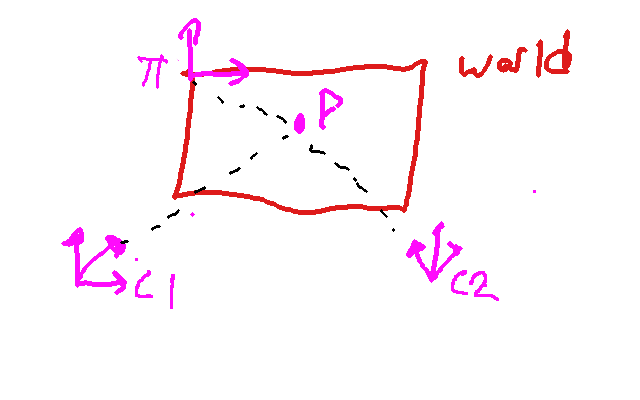
\includegraphics[page=1,width=0.75\textwidth]{q1_1a}
\caption{ Camera Frames observing point on plane } 
\label{fig:autoencout}
\end{figure}   


\subsection{Q1.2}

%%%%%%%%%5
In section 1.1, we proved that a 3x3 homography matrix $\textbf{H}$ exists to map a point on a plane in the world frame from one image plane to another. Part of that process involves using the camera projetion matrices M1 and M2. These matrices are a function of intrinsic camera parameters and external world reference parameters.
The same applies here, except that M1 must be derived as  
$$
\textbf{M}_{1} = 
\textbf{K}_{1} 
\begin{bmatrix}
\textbf{I} & \textbf{0}
\end{bmatrix}
$$
And M2 derived as
$$
\textbf{M}_{2} = 
\textbf{K}_{2} 
\begin{bmatrix}
\textbf{R} & \textbf{0}
\end{bmatrix}
$$

With M1 and M2 in hand, the proof in section 1.1 shows that $\textbf{H}$ exists.

\subsection{Q1.3}
\subsubsection{Q1.3.1}
Consider a transform matrix H that maps a point from one image plane to another image plane. Ignoring all other frames ( camera , world, or otherwise ) , 6 degrees of freedom are required to describe the rotation and translation from one frame to another (3 for translation, 3 for rotation). In the case of cameras, changes in focal length will create a scaling effect in the X and Y directions, which amounts to 2 degrees of freedom. All in, that H has 8 degrees of freedom.
\subsubsection{Q1.3.2}
Each image point contains two pieces of information. 4 points are therefore required to solve for the transformation matrix described in the preceeding subsection.
\subsubsection{Q1.3.3}
$$
\textbf{x}^{i}_{1}=
\begin{bmatrix}
x^{ \prime } \\ y ^ { \prime } \\ 1
\end{bmatrix}
$$

$$
\textbf{x}^{i}_{2}=
\begin{bmatrix}
x \\ y \\ 1
\end{bmatrix}
$$

$$
\textbf{x}^{i}_{1}=
\alpha
\textbf{H}
\textbf{x}^{i}_{2}
=
\alpha
\begin{bmatrix}
h_{11} & h_{12} & h_{13} \\
h_{21} & h_{22} & h_{23} \\
h_{31} & h_{32} & h_{33} 
\end{bmatrix}
\textbf{x}^{i}_{2}
$$

$$
\textbf{x}^{i}_{1}=
\begin{bmatrix}
x^{ \prime } \\ y ^ { \prime } \\ 1
\end{bmatrix}
=
\begin{bmatrix}
\alpha ( h_{11} x + h_{12} y + h_{13} ) \\
\alpha ( h_{21} x + h_{22} y + h_{23} ) \\
\alpha ( h_{31} x + h_{32} y + h_{33} )
\end{bmatrix}
$$

$$
\begin{bmatrix}
( h_{31} x + h_{32} y + h_{33} ) x^{ \prime } \\ 
( h_{31} x + h_{32} y + h_{33} ) y^ { \prime } 
\end{bmatrix}
=
\begin{bmatrix}
( h_{11} x + h_{12} y + h_{13} ) \\
( h_{21} x + h_{22} y + h_{23} )
\end{bmatrix}
$$

$$
\begin{bmatrix}
( h_{31} x + h_{32} y + h_{33} ) x^{ \prime } - ( h_{11} x + h_{12} y + h_{13} ) \\
( h_{31} x + h_{32} y + h_{33} ) y^{ \prime } - ( h_{21} x + h_{22} y + h_{23} )
\end{bmatrix}
=
\begin{bmatrix}
0 \\ 0
\end{bmatrix}
$$

$$
\begin{bmatrix}
- h_{11} x 
- h_{12} y 
- h_{13}
+ 0 + 0 + 0
+ h_{31} x  x^{ \prime }
+ h_{32} y  x^{ \prime }
+ h_{33} x^{ \prime }   \\
0 + 0 + 0
- h_{21} x 
- h_{22} y 
- h_{23}
+ h_{31} x y^{ \prime } 
+ h_{32} y y^{ \prime } 
+ h_{33}   y^{ \prime } 
\end{bmatrix}
=
\begin{bmatrix}
0 \\ 0
\end{bmatrix}
$$

$$
\textbf { h } = 
\begin{bmatrix}
h_{11} & h_{12} & h_{13} & h_{21} & h_{22} & h_{23} & h_{31} & h_{32} & h_{33} 
\end{bmatrix}^{T}
$$

$$
\textbf{A}_{i} = 
\begin{bmatrix}
- x 
- y 
- 1
+ 0 + 0 + 0
+ x  x^{ \prime }
+ y  x^{ \prime }
+ x^{ \prime }   \\
0 + 0 + 0
- x 
- y 
- 1
+ x y^{ \prime } 
+ y y^{ \prime } 
+   y^{ \prime } 
\end{bmatrix}
=
\begin{bmatrix}
0 \\ 0
\end{bmatrix}
$$

$$
\textbf{A}_{i} 
\textbf { h } =  \textbf { 0 }
$$


\subsection{Q1.4}
Consider a camera with static intrinsic parameters. If the camera is rotated around it's center C ( origin of the camera frame ), then the homography matrix $\textbf{H}$ simply defines a rotation around C. If  $\textbf{H}$ is parameterized by an angle $\theta$, then rotating by $\theta$ twice ( $2 \theta$ ) is the same as multiplying by $\textbf{H}$ twice which is simply $\textbf{H}^{2}$.

\subsection{Q1.5}
Planar homography fails in cases where points are obfuscated in some views and visible in others. Planar homography also relies on the existence of some plane exists in an image, which is not a guarantee.
\subsection{Q1.6}

\section{Q2}
\section{Q2.5}
To test how BRIEF feature mapping works under rotation, I created a script that rotates an image and checks the feature matching every 10 degrees ( matches verified visually ). The number of correct matches is shown against the rotation in Figure \ref{fig:imgrot}.
\begin{figure}[H]
\centering
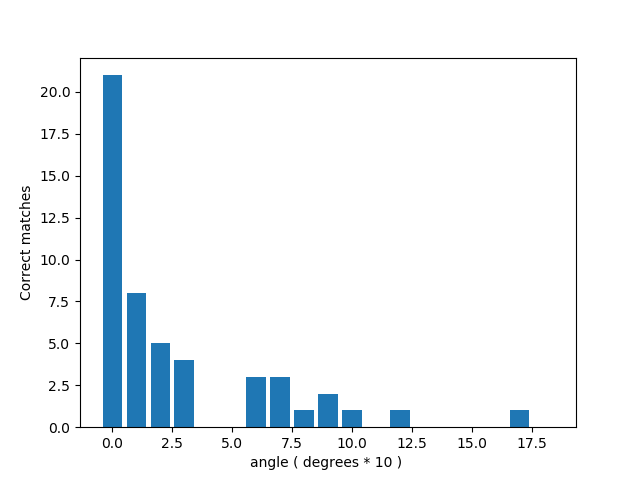
\includegraphics[page=1,width=0.75\textwidth]{q2_5}
\caption{ Correct point matches vs. image rotation } 
\label{fig:imgrot}
\end{figure}   


\section { Q2 }
\subsection { Q2.4.1 }

Figure \ref{fig:plotmatch} shows descriptor matches for two similar images of soup. Matching fails when image patches corresponding to different physical features contain similar descriptor information.

\begin{figure}[H]
\centering
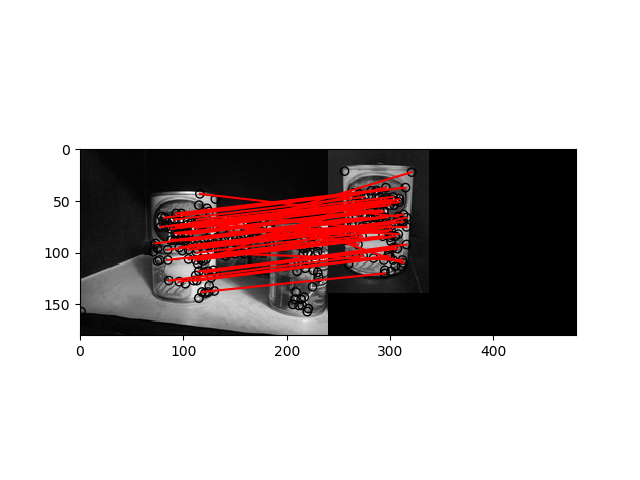
\includegraphics[page=1,width=0.75\textwidth]{q2_4}
\caption{ No soup for you }
\label{fig:plotmatch}
\end{figure}   

\subsection { Q2.5 }

So far, these BRIEF descriptors have been working well. But how do they operate under rotation? Let's find out! I took an image and tested matches against itself while holding the first instance fixed and rotating the second instance in 10 degree increments from 0 to 180 degrees. I counted matches manually using my human neural network as ground truth, and adjusted thresholding so that fewer matches were produced. Figure \ref{fig:rotbad} shows a histogram of succesful descriptor matches. The histogram shows that fewer correct matches are found as rotation is increased, so BRIEF is not rotation invariant.

\begin{figure}[H]
\centering
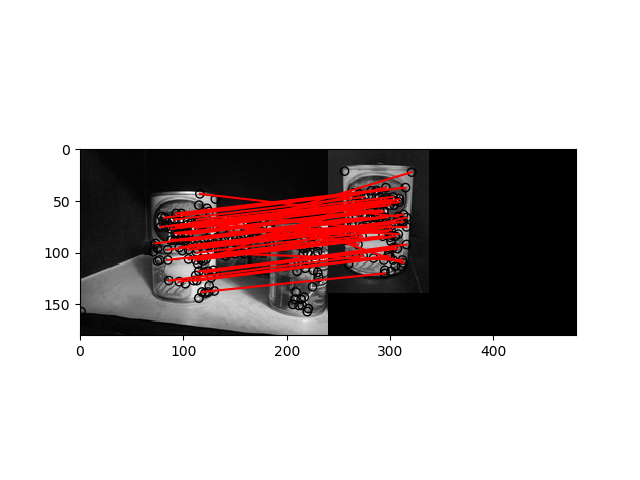
\includegraphics[page=1,width=0.75\textwidth]{q2_4}
\caption{ Drop it down, flip it and reverse it }
\label{fig:rotbad}
\end{figure}   


\section { Q3 }
Figure \ref{fig:lumos} shows the cover of a Harry Potter book mapped and overlayed onto a book on a desk.
\begin{figure}[H]
\centering
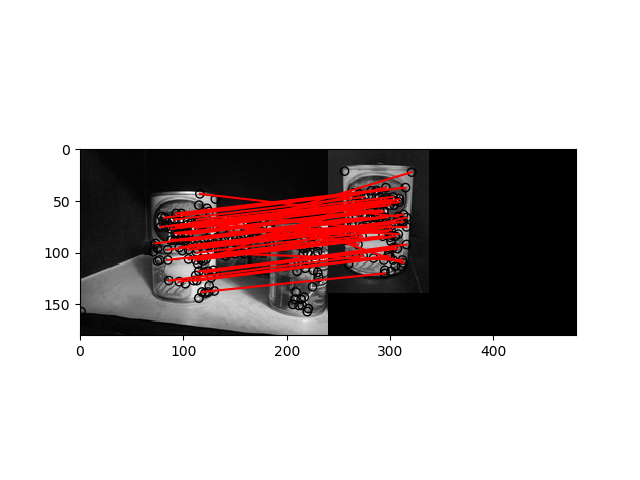
\includegraphics[page=1,width=0.75\textwidth]{q2_4}
\caption{ Harry Potter book cover mapped to CV book on desk }
\label{fig:lumos}
\end{figure}   

The result homography matrix is shown below:
$$
H = 
\begin {bmatrix} 
2.376   &  0.714  & -696.798 \\
547.627 &  4.400  & -859.204 \\
0.00005 &  0.004  & 1.000
\end {bmatrix} 
$$

\section { Q4 }
\subsection { Q4.1 }
Figure \ref{fig:q41} shows two images taken from a baseball stadium of a skyline merged together into a panorama.
The resulting homography matrix is shown below:
$$
H = 
\begin {bmatrix}
1.36e+00  & -3.21e-03 & -1.42e+02 //
1.54e-01  &  1.20e+00 & -6.97e+00 //
1.85e-03  & -1.61e-04 &  1.00e+00
\end {bmatrix}
$$

\begin{figure}[H]
\centering
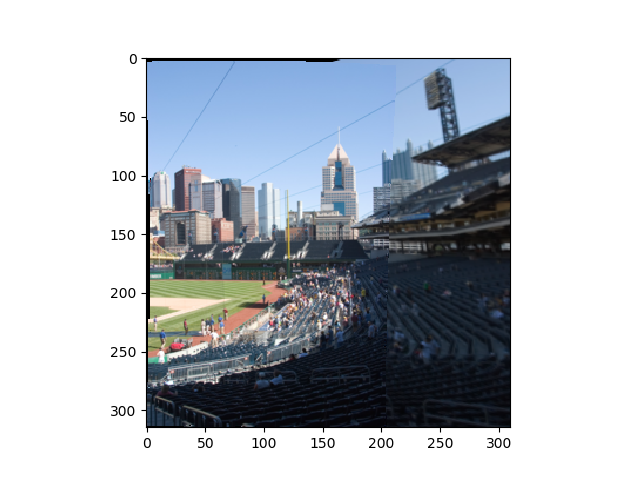
\includegraphics[page=1,width=0.75\textwidth]{q4_1}
\caption{ Image 2 warped and overlayed on Image 1 }
\label{fig:q41}
\end{figure}   

\subsection { Q4.2 }
Figure \ref{fig:q42} shows the same two images used in Q4.1 stitched together, with the addition of a feature to automatically control the output shape of the image such that the output image contains the entirety of both images.

\begin{figure}[H]
\centering
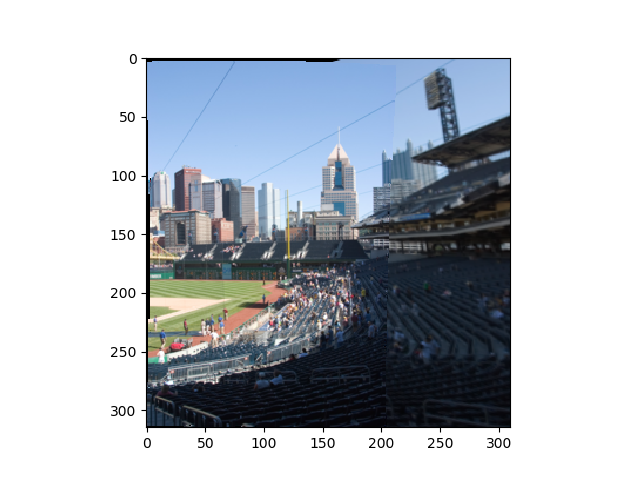
\includegraphics[page=1,width=0.75\textwidth]{q4_1}
\caption{ Stitched images without clipping}
\label{fig:q42}
\end{figure}   

\subsection { Q4.3 }
The function created for the previous section was wrapped in a high level function that extracts correspondences, computes homographies, and stitches images. Images incline\_L and incline\_R were stitched together, shown in figure \ref{fig:q4_3}.
T
The resulting homography matrix is shown below:
$$
H = 
\begin {bmatrix}
1.49e+00 &  3.26e-02 & -5.33e+02 //
1.55e-01 &  1.27e+00 & -1.17e+01 //
5.64e-04 & -8.95e-05 &  1.00e+00
\end {bmatrix}
$$

\begin{figure}[H]
\centering
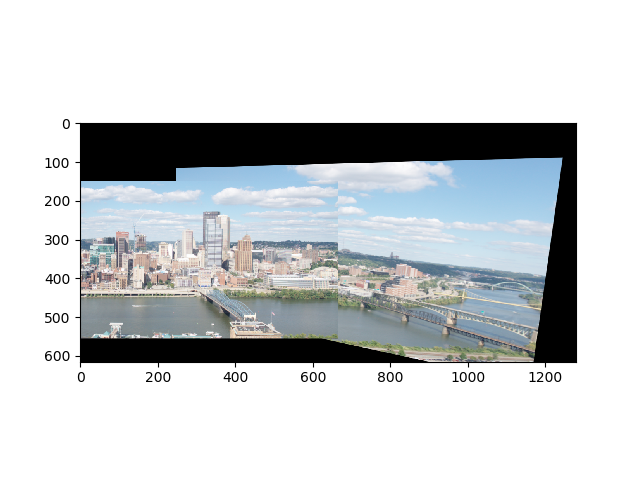
\includegraphics[page=1,width=0.75\textwidth]{q4_3}
\caption{ Automagic panorama of skyline}
\label{fig:q42}
\end{figure}   



\end{document}
